\chapter{Transformer-Architektur im Detail}

Im ursprünglichen Werk \textit{Attention Is All You Need}, in dem das grundlegende Transformer-Architektur vorgestellt wurde, besteht ein Transformer aus zwei Hauptmodulen: dem Encoder und dem Decoder (vgl. \cite[S. 3]{attention}).
Um die Architektur eines Transformers besser zu verstehen, müssen zunächst die Komponenten betrachtet werden, die in Encoder und Decoder eingesetzt werden.

\section{Multi-Head-Attention}

Wie schon im vorherigen Kapitel beschrieben, ist \enquote{Scaled Dot-Product Attention} ein zentraler Baustein in der Transformer-Architektur.  
Um Transformer noch effizienter zu gestalten, wird Scaled Dot-Product Attention in Form der \textbf{Multi-Head-Attention} angewendet. 
Dabei beschreibt jeder einzelne Kopf einen eigenen Attention-Zyklus, wie oben beschrieben (vgl. \cite[S. 211]{paass.2020}).

Jeder Kopf verwendet unterschiedliche Gewichtungsmatrizen, um den Fokus bei der Analyse der Zusammenhänge zwischen Tokens auf verschiedene Schwerpunkte zu setzen (vgl. \cite[S. 5]{attention}).  
So kann beispielsweise ein Kopf die Tokens hinsichtlich syntaktischer Beziehungen analysieren, während ein anderer die semantischen Beziehungen betrachtet.  
Für jeden Attention-Kopf \( h \) werden dabei unterschiedliche Gewichtungsmatrizen \( \mathbf{W}_{Qh} \), \( \mathbf{W}_{Kh} \) und \( \mathbf{W}_{Vh} \) verwendet.

Nach der parallelen Verarbeitung werden die jeweiligen Ergebnisse der Köpfe zusammengefügt (auch als Konkatenieren bezeichnet) und mit Hilfe einer weiteren Gewichtungsmatrix \( \mathbf{W}_{O} \) zusammengefasst (vgl. \cite[S. 5]{attention}).  
\( \mathbf{W}_{O} \) ist die Matrix, welche die Ergebnisse der Attention-Köpfe unterschiedlich gewichtet.  
Umgangssprachlich formuliert bildet sie eine einheitliche Schlussfolgerung für den Transformer aus dem Multi-Head-Attention-Zyklus.

\section{Positional Encodings}

Ein Problem bei der einfachen Verwendung von Scaled Dot-Product Attention ist, dass die tatsächliche Reihenfolge der Tokens verloren geht.  
Der Grund dafür ist, dass bei dem Attention-Algorithmus alle Zusammenhänge zwischen Token parallel ermittelt werden und nicht Wort für Wort (vgl. \cite[S. 6]{attention}).   
Das Ergebnis ist somit unabhängig von der Reihenfolge der Tokens.
Der Algorithmus kommt so für die Wortfolge \enquote{Katze jagt Hund} und \enquote{Hund jagt Katze} zum den gleichen Ergebnis, obwohl die semantische Bedeutung offensichtlich eine andere ist. 

Hier kommt das \textbf{Positional Encoding} ins Spiel.  
Dabei werden zu den ursprünglichen Embeddings, die aus den Tokens generiert wurden, Positionsdaten hinzugefügt, die der Transformer erkennen kann (vgl. \cite[S. 6]{attention}).  
Hierfür verwendet man abwechselnd Sinus- und Cosinus-Funktionen:

\[
PE_{(pos, 2i)} = \sin\left(\frac{\text{pos}}{10000^{\frac{2i}{d_{\text{model}}}}}\right), \quad
PE_{(pos, 2i+1)} = \cos\left(\frac{\text{pos}}{10000^{\frac{2i}{d_{\text{model}}}}}\right)
\]

Hierbei ist \( \text{pos} \) die Position des Tokens in der Wortfolge, \( i \) ist die aktuell zu betrachtende Dimension für diesen Token, und \( d_{\text{model}} \) ist die Anzahl der Dimensionen im Model.

Die unterschiedlichen Frequenzen der Sinus- und Cosinus-Funktionen ermöglichen es, dass jede Dimension des Embeddings anders auf die Position reagiert.  
Sinus und Cosinus haben eine periodische Struktur, die es dem Transformer erlaubt, die Position der Tokens in der ursprünglichen Eingabe sowie die Positionsunterschiede zwischen Tokens zu ermitteln.  
Die abwechselnde Verwendung dieser Funktionen sorgt dafür, dass sie sich nie überlagern und somit unabhängige Informationen darstellen (vgl. \cite[S. 208]{paass.2020}).

\section{Addition und Normalisierung}

Die Addition-und-Normalisierung-Komponente bewahrt originale Eingabeinformationen, die durch die schrittweise Verarbeitung im Transformer verloren gehen könnten. 
Nach jeder Verarbeitung, beispielsweise durch die Multi-Head-Attention, werden die Ausgabewerte mit den ursprünglichen Eingabewerten \( x_i \) addiert . 
Dadurch stehen auch für nachfolgende Komponenten die Originalinformationen weiterhin zur Verfügung (vgl. \cite[K. 3]{layernorm}).

\[
z_i = x_i + \text{SubkomponentenOutput}_i
\]

Bei der Normalisierung wird berechnet, wie viele Standardabweichungen ein Wert \( z_i \) vom Mittelwert entfernt ist. 
Dadurch werden die Werte standardisiert, indem die Verteilung zentriert (Mittelwert \( \mu \) wird 0) und skaliert (Standardabweichung \( \sigma \) wird 1) wird. 
Anschließend werden die Werte abhängig vom Modelltraining durch Streckung (mit \( \gamma \)) und Verschiebung (mit \( \beta \)) angepasst (vgl. \cite[K. 3]{layernorm}). 
Diese Anpassung macht die Normalisierung flexibel und trainierbar.

\[
\hat{z}_i = \frac{z_i - \mu}{\sigma}
\]
\[
y_i = \gamma \cdot \hat{z}_i + \beta
\]

\section{Feed-Forward-Schicht}

Während \textbf{Multi-Head-Attention} lineare Zusammenhänge zwischen Tokens berechnet, benötigt der Transformer eine zusätzliche Komponente, um nicht-lineare Zusammenhänge zu erfassen. 
Hierfür wird die \textbf{Feed-Forward-Schicht} verwendet, die die addierten und normalisierten Ergebnisse aus der Multi-Head-Attention-Schicht weiterverarbeitet (vgl. \cite[S. 5]{attention}).

Die Feed-Forward-Schicht ist ein neuronales Netzwerk, das aus zwei linearen Transformationen mit einer nicht-linearen Aktivierungsfunktion in der Mitte besteht.
Im ersten Schritt wird die Eingabematrix mit der Gewichtungsmatrix \( W_1 \) multipliziert, was die erste Schicht des neuronalen Netzes darstellt. Dabei entsteht eine Matrix mit viermal so vielen Dimensionen wie der Eingabematrix, die anschließend um einen Bias-Wert \( b_1 \) erweitert wird.
Danach wird die erste Schicht durch die nicht-lineare Aktivierungsfunktion \textbf{ReLU} (eng. Rectified Linear Unit) mit der zweiten Schicht verbunden (vgl. \cite[S. 212]{paass.2020}). 
Die ReLU-Funktion hat eine einfache nicht-lineare Eigenschaft: Wenn ein Eingabewert negativ ist, wird er zu 0; wenn er positiv ist, bleibt er unverändert und es bleibt bei einem linearen Zusammenhang:

\[
\text{ReLU}(x) = \max(0, x)
\]

Somit werden nur die positiven Werte in der weiteren Verarbeitung berücksichtigt.

In der zweiten Schicht werden die Werte aus der ReLU-Funktion mit der zweiten Gewichtungsmatrix \( W_2 \) multipliziert und somit wieder auf die ursprüngliche Eingabegröße skaliert. 
Auch hier wird der resultierende Vektor durch einen Bias-Wert \( b_2 \) ergänzt (vgl. \cite[S. 5]{attention}).
Insgesamt kann die Feed-Forward-Schicht mathematisch so ausgedrückt werden: 
\[
\text{Feed-Forward}(x) = \text{ReLU}(W_1 x + b_1) W_2 + b_2
\]

\section{Encoder}

Der \textbf{Encoder} übersetzt die Eingabewörter in eine abstrahierte Repräsentation (vgl. \cite[S. 3]{attention}).  
Ziel ist es hierbei, die semantischen und syntaktischen Informationen des Textes zu extrahieren und zu kodieren.  

Am Beginn jeder Textverarbeitung wird, wie auch im vorherigem Kapitel beschrieben, der Eingabetext tokenisiert und in Embeddings umgewandelten.
Anschließend werden einmalig Positional-Encodings hinzugefügt, die Positionsdaten der Tokens im Eingabetext ergänzen.

Nun werden diese Embedding-Informationen an die erste Encoder-Schicht weitergeleitet.
Es sind mehrere Encoder-Schichten in einem Transformer implementiert (vgl. \cite[S. 3]{attention}). 
In einer Encoder-Schicht wird zunächst Multi-Head-Attention angewendet.
Das Ergebnis der Multi-Head-Attention, also die relevanten, weiterzuanalysierenden Informationen über Tokens werden mit den ursprünglichen Eingabe-Embeddings der Encoder-Schicht der Addition und Normalisierung unterzogen.

Im zweiten Teil der Encoder-Schicht werden die Werte dann mit Feed-Forward-Komponente weiterverarbeitet (vgl. \cite[S. 3]{attention}).
Am Schluss werden diese weiterverarbeiteten Werte nocheinmal mit den Werten vor der Feed-Forward-Komponente addiert und normalisiert. 
Nun werden die Werte an die nächste Encoder-Schicht weitergegeben, welche die Prozedur wiederholt.

Nach der letzten Schicht liefert der Encoder eine kontextbewusste Darstellung der Eingabesequenz, in der jedes Token nicht nur seine ursprüngliche Bedeutung, sondern auch die relevanten Zusammenhänge mit anderen Tokens der Sequenz berücksichtigt (vgl. \cite[S. 3]{attention}).
Nun können diese Informationen an den Decoder weitergegeben werden.

\section{Decoder}

Der \textbf{Decoder} ist die zweite Komponente des Modells und nutzt die abstrahierte Repräsentation des Encoders, um passende Outputs zu generieren (vgl. \cite[S. 3]{attention}). 
In jeder Iteration berechnet er das nächste Token, das zum Output hinzugefügt werden soll, wobei er den zuletzt generierten Token als zusätzlichen Kontext berücksichtigt.

Zu Beginn eines Decoder-Zyklus wird, analog zum Encoder, der Eingabetext in Embeddings umgewandelt und mithilfe des Positional Encodings mit Positionsinformationen angereichert  (vgl. \cite[S. 213]{paass.2020}). 
Der Unterschied liegt jedoch darin, dass der Eingabetext in der ersten Iteration des Decoders nur aus einem \enquote{Start-Token} besteht, da noch keine weiteren Tokens generiert wurden. 
Diese initialen Embeddings werden dann an die Decoder-Schichten weitergeleitet, wo die eigentliche Verarbeitung stattfindet.

Im ersten Schritt jeder Decoder-Schicht wird eine spezielle Variante von Multi-Head-Attention angewendet: die \textbf{Masked Multi-Head Attention} (vgl. \cite[S. 213]{paass.2020}). 
Hierbei werden zukünftige Tokens durch eine Maske verdeckt, sodass der Decoder nur bereits generierte Tokens verwenden kann. 
Dies verhindert, dass der Decoder Informationen vorwegnimmt.  
Während des Trainings wird der Decoder mit der gesamten Zielsequenz versorgt, wobei durch Maskierung nur bereits bekannte Tokens sichtbar sind. 
Dies simuliert den schrittweisen Vorhersageprozess.  
Die Ergebnisse der Masked Multi-Head Attention werden anschließend mit den ursprünglichen Eingabewerten addiert und normalisiert.

Im zweiten Schritt wird erneut Multi-Head Attention angewendet, allerdings in einer modifizierten Form, die als \textbf{Cross-Attention} bezeichnet wird (vgl. \cite[S. 212]{paass.2020}). 
Hier werden die Queries (\( Q \)) regulär aus den Embeddings des Decoders berechnet, während die Keys (\( K \)) und Values (\( V \)) aus den Ergebnissen des Encoders stammen. 
Durch die separaten \( K \) und \( V \) aus dem Encoder kann der Decoder die im Eingabetext gespeicherten Kontextinformationen nutzen, um die Ausgabe gezielt zu steuern. 
Dies ist besonders wichtig, wenn der Eingabetext viele Details enthält, die in der Antwort berücksichtigt werden müssen.  
Die Ergebnisse der Cross-Attention werden ebenfalls addiert und normalisiert.

Im dritten Schritt durchlaufen die Werte eine Feed-Forward-Schicht, die die Berechnungen weiter verfeinert (vgl. \cite[S. 3]{attention}). 
Auch hier folgt eine Addition mit den ursprünglichen Werten und eine Normalisierung.

Die resultierenden Embeddings werden entweder an die nächste Decoder-Schicht weitergeleitet, um den Prozess zu wiederholen, oder sie werden für die Ausgabe vorbereitet (vgl. \cite[S. 213]{paass.2020}). 
Bei der Ausgabe wird jedes Embedding einem Token aus dem Vokabular zugeordnet, das als ganze natürliche Zahl dargestellt wird. 
Anschließend berechnet die Softmax-Funktion die Wahrscheinlichkeiten für alle möglichen Tokens und erzeugt dabei eine Wahrscheinlichkeitsverteilung über das gesamte Vokabular. 
Das Token mit der höchsten Wahrscheinlichkeit wird ausgewählt und zur finalen Ausgabe hinzugefügt (vgl. \cite[S. 213]{paass.2020}). 
Dieses neue Token wird dann als Eingabe in den nächsten Decoder-Zyklus eingespeist. 
Der Vorgang wird fortgesetzt, bis der Decoder ein \enquote{End of Sequence}-Token (\textit{EOS}) generiert, das das Ende der Ausgabe markiert.



\begin{figure}[ht]
	\centering
	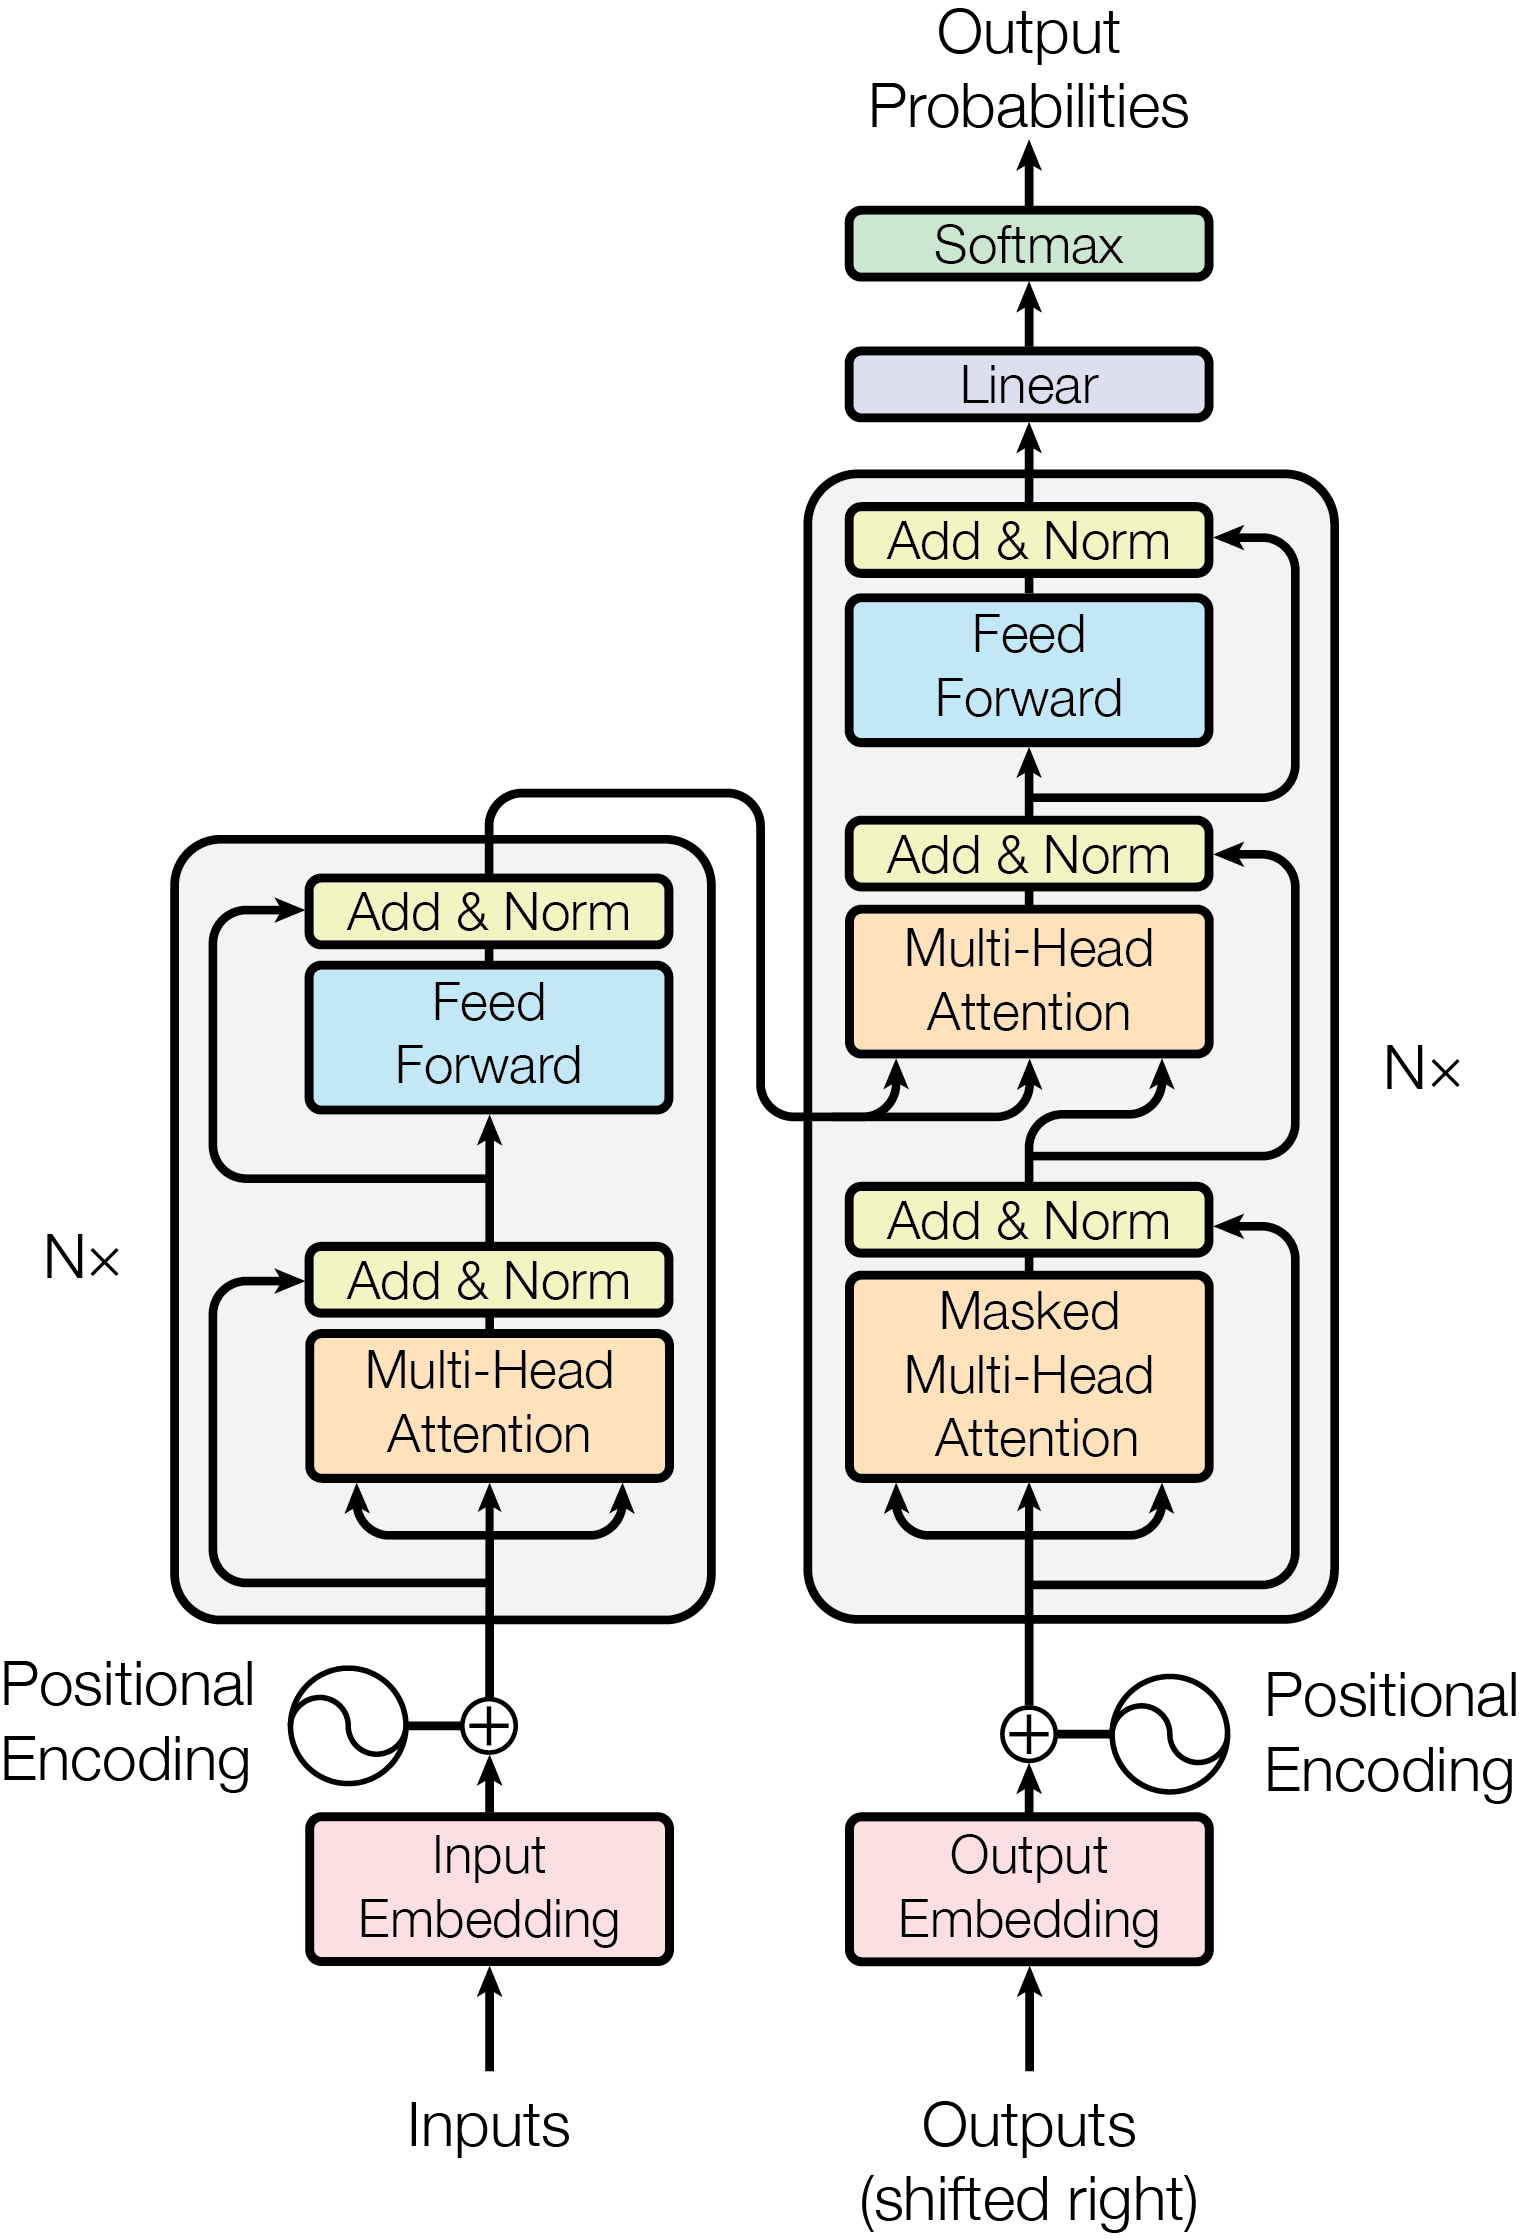
\includegraphics[width=0.6\textwidth]{Bilder/ModalNet-21.png} 
	\caption{Tranformer-Architektur aus \cite[S. 3]{attention}}
	\label{fig:scaled-dot}
\end{figure}